\section{Экспериментальная часть}
\subsection{Эксперимент для проверки точности измерения времени}
Для проверки точности измерения времени проведём следующий эксперимент.

Сгенерируем семейство программ, которые не делают ничего, кроме вызова функции стандартной библиотеки \textit{C} \textit{usleep}. Аргументами функции будет число $10^n$, где $n$ --- число от 1 до 6 включительно. Таким образом, после запуска программа устанавливает таймер на заданное число микросекунд (от 1 мкс до 1000000 мкс = 1 с), останавливается и после его срабатывания завершает работу.

Далее на рис. \ref{img:calibration} приведён график измеренного времени исполнения семейства таких программ и «реального» времени их выполнения --- т.е. времени, указанного в аргументе функции, создающей таймер. График построен с помощью инструментария в автоматическом режиме.

\begin{figure}[H]
    \center{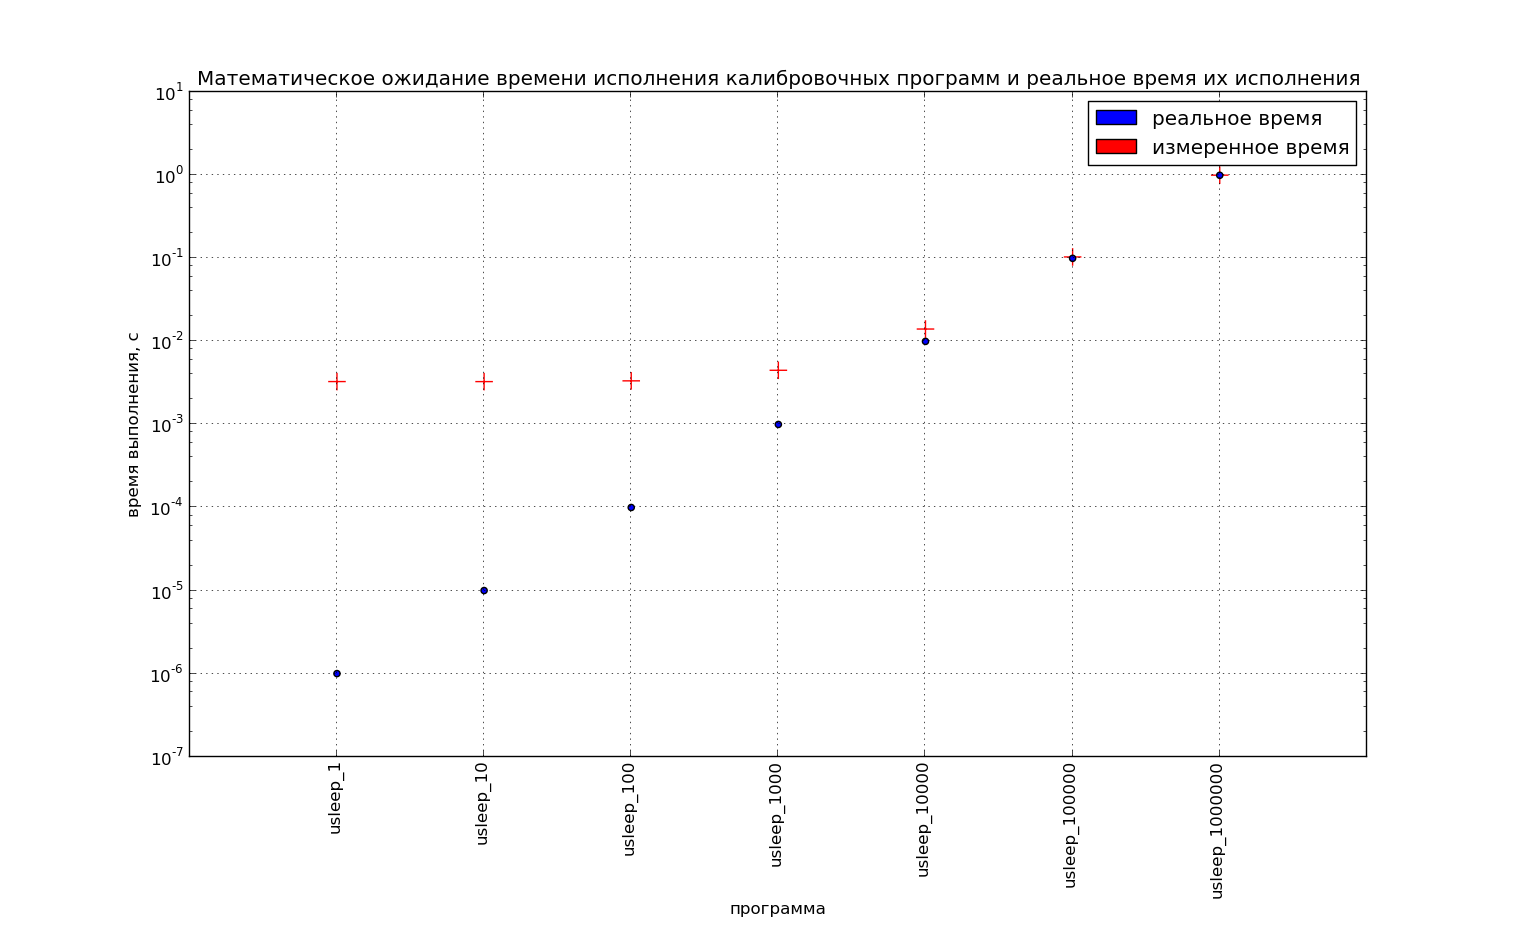
\includegraphics[width=1\linewidth]{calibration}}
    \caption{График времени измеренного исполнения семейства калибровочных программ.}
    \label{img:calibration}
\end{figure}

Как мы видим на рис. \ref{img:calibration}, измеренное время асимптотически приближается к значению между $10^{-2}$ и $10^{-3}$ --- около 0,005.

Далее на рис. \ref{img:default_calibration} приведён текстовый вывод результата описанного эксперимента из инструментария.
\begin{figure}[H]
    \fontsize{10}{12}
    \begin{verbatim}
        Experiment performed:
            Real time: 0.000001
            Measured time: 0.000531
            Relative error: 530.11
        
        Experiment performed:
            Real time: 0.000010
            Measured time: 0.000498
            Relative error: 48.79
        
        Experiment performed:
            Real time: 0.000100
            Measured time: 0.000795
            Relative error: 6.95
        
        Experiment performed:
            Real time: 0.001000
            Measured time: 0.001499
            Relative error: 0.50
        
        Experiment performed:
            Real time: 0.010000
            Measured time: 0.010893
            Relative error: 0.09
        
        Experiment performed:
            Real time: 0.100000
            Measured time: 0.101603
            Relative error: 0.02
        
        Experiment performed:
            Real time: 1.000000
            Measured time: 1.001015
            Relative error: 0.00
    \end{verbatim}
    \caption{Вывод инструментария для описываемого эксперимента.}
    \label{img:default_calibration}
\end{figure}